\chapter{Going Large-Scale}
\label{chap:stm}

In this chapter we present a technique which allows to scale the approach of functional ABS as presented in the paper in Appendix \ref{app:pfe} to massively large-scale simulations. This is a very recent development which didn't make it into the paper but will make an appearance in the final thesis in the form inspired by this chapter. Due to the increasing need for massively large-scale ABS in recent years \cite{lysenko_framework_2008}, making this possible with our functional approach as well, gives our research a much larger impact.

The whole concept of our approach is built on the usage of Software Transactional Memory (STM), which we will introduce in Section \ref{sect:stm_intro}, where we follow the main paper \cite{harris_composable_2005} on STM \footnote{We also make use of the excellent tutorial \url{http://book.realworldhaskell.org/read/software-transactional-memory.html}.}. In Section \ref{sect:stm_impl} we give a short overview of our implementation, presenting and discussing code. In Section \ref{sect:stm_perf} we present performance comparisons and discuss the implications more in-depth in Section \ref{sect:stm_discussion}. Finally we will give a short outline over further research in \ref{sect:stm_further}.

\section{Introduction}
\label{sect:stm_intro}
Concurrent programming is notoriously difficult to get right, the difficulty of reasoning about the interactions of multiple concurrently running threads and low level operational details of synchronisation primitives and locks. The main problems are:

\begin{itemize}
	\item Race conditions due to forgotten locks.
	\item Deadlocks resulting from inconsistent lock ordering.
	\item Corruption caused by uncaught exceptions.
	\item Lost wakeups induced by omitted notifications.
\end{itemize}

Worse, concurrency does not compose. It is utterly difficult to write two functions (or methods in an object) which act on concurrent data, one can compose into a larger concurrent function because one has to know about their internal details of locking, which breaks encapsulation and makes composition depend on knowledge about their implementation. Also it is impossible to compose two functions e.g. where one withdraws some amount of money from an account and the other deposits this amount of money into a different account: one ends up with a temporary state where the money is in none of either accounts, creating an inconsistency - a potential source for errors because threads can be rescheduled at any time.

STM promises to solve all these problems for a very low cost. In STM one executes actions atomically where modifications made in such an action are invisible to other threads until the action is performed. Also the thread in which this action is run, doesn't see changes made by other threads - thus execution of STM actions are isolated. When a transaction exists one of the following things will occur:

\begin{enumerate}
	\item If no other thread concurrently modified the same data as us, all of our modifications will simultaneously become visible to other threads.
	\item Otherwise, our modifications are discarded without being performed, and our block of actions is automatically restarted.
\end{enumerate}

Note that the ability to \textit{restart} a block of actions without any visible effects is only possible due to the nature of Haskells type-system which allows being explicit about side-effects: by restricting the effects to STM only ensures that no uncontrolled effects, which cannot be rolled-back, occur.

STM is implemented using optimistic synchronisation. This means that instead of locking access to shared data, each thread keeps a transaction log for each read and write to shared data it makes. When the transaction exists, this log is checked whether other threads have written to memory it has read - it checks whether it has a consistent view to the shared data or not. This might look like a serious overhead but the implementations are very mature by now, being very performant and the benefits outweigh its costs by far.

Applying this to our agents is very simple: because we already use Dunai / BearRiver as our FRP library, we can run in arbitrary Monadic contexts. This allows us to simply run agents within an STM Monad and execute each agent in their own thread. This allows then the agents to communicate concurrently with each other using the STM primitives without problems of explicit concurrency, making the concurrent nature of an implementation very transparent. Further through optimistic synchronisation we should arrive at a much better performance than with low level locking.

\subsection{STM primitives}
STM comes with a number of primitives to share transactional data. Amongst others the most important ones are:

\begin{itemize}
	\item TVar - A transactional variable which can be read and written arbitrarily. 
	\item TArray - A transactional array where each cell is an individual shared data, allowing much finer-grained transactions instead of e.g. having the whole array in a TVar.
	\item TChan - A transactional channel, representing an unbounded FIFO channel.
	\item TMVar - A transactional \textit{synchronising} variable which is either empty of full. To read from an empty or write to a full TMVar will cause the current thread to retry its transaction.
\end{itemize}

Additionally, the following functions are provided:

\begin{itemize}
	\item atomically :: STM a $\to$ IO a - Performs a series of STM actions atomically. Note that we need to run this in the IO Monad, which is obviously required when running an agent in a thread.
	\item retry :: STM a - Allows to retry a transaction immediately.
	\item orElse :: STM a $\to$ STM a $\to$ STM a - Tries the first STM action and if it retries it will try the second one. If the second one retries as well, orElse as a whole retries.
\end{itemize}

\section{Implementation}
\label{sect:stm_impl}
For a proof-of-concept we changed the reference implementation of the agent-based SIR model on a 2D-grid as described in the paper in Appendix \ref{app:pfe}. In it, a State Monad is used to share the grid across all agents where all agents are run after each other to guarantee exclusive access to the state. We replaced the State Monad by the STM Monad, share the grid through a \textit{TVar} and run every agent within its own thread. All agents are run at the same time but synchronise after each time-step which is done through the main-thread.

We make STM the innermost Monad within a RandT transformer:
\begin{HaskellCode}
type SIRMonad g   = RandT g STM
type SIRAgent g   = SF (SIRMonad g) () ()
\end{HaskellCode}

In each step we use an \textit{MVar} to let the agents block on the next $\Delta t$ and let the main-thread block for all results. After each step we output the environment by reading it from the \textit{TVar}:
\begin{HaskellCode}
-- this is run in the main-thread
simulationStep :: TVar SIREnv
               -> [MVar DTime]
               -> [MVar ()]
               -> Int
               -> IO SIREnv
simulationStep env dtVars retVars _i = do
  -- tell all threads to continue with the corresponding DTime
  mapM_ (`putMVar` dt) dtVars
  -- wait for results, ignoring them, only [()]
  mapM_ takeMVar retVars
  -- read last version of environment
  readTVarIO env
\end{HaskellCode}

Each agent runs within its own thread. It will block for the posting of the next $\Delta t$ where it then will run the MSF stack with the given $\Delta t$ and atomically transacting the STM action. It will then post the result of the computation to the main-thread to signal it has finished. Note that the number of steps the agent will run is hard-coded and comes from the main-thread so that no infinite blocking occurs and the thread shuts down gracefully.

\begin{HaskellCode}
createAgentThread :: RandomGen g 
                  => Int 
                  -> TVar SIREnv
                  -> MVar DTime
                  -> g
                  -> (Disc2dCoord, SIRState)
                  -> IO (MVar ())
createAgentThread steps env dtVar rng0 a = do
    let sf = uncurry (sirAgent env) a
    -- create the var where the result will be posted to
    retVar <- newEmptyMVar
    _ <- forkIO (sirAgentThreadAux steps sf rng0 retVar)
    return retVar
  where
    agentThread :: RandomGen g 
                => Int
                -> SIRAgent g
                -> g
                -> MVar ()
                -> IO ()
    agentThread 0 _ _ _ = return ()
    agentThread n sf rng retVar = do
      -- wait for next dt to compute next step
      dt <- takeMVar dtVar

      -- compute next step
      let sfReader = unMSF sf ()
          sfRand   = runReaderT sfReader dt
          sfSTM    = runRandT sfRand rng
      ((_, sf'), rng') <- atomically sfSTM 
      
      -- post result to main thread
      putMVar retVar ()
      
      agentThread (n - 1) sf' rng' retVar
\end{HaskellCode}

The implementation of the susceptible, infected and recovered agents are the same except that instead of accessing the environment through \textit{get} and \textit{put}, we use \textit{readTVar}, \textit{writeTVar} and \textit{modifyTVar}.

\section{Performance Comparison}
\label{sect:stm_perf}
The model we use in the experiments is the agent-based SIR model on a 51 x 51 grid (single infected at center), stepped with $\Delta t = 0.1$ until virtual simulation time $t=100$. We compared three different experiments:

\begin{enumerate}
	\item State Monad: the reference implementation of the paper in Appendix \ref{app:pfe} using a State Monad to share the grid across all agents.
	\item STM Single-Core: the implementation of Section \ref{sect:stm_impl}, running on a single core.
	\item STM 4-Core: the implementation of Section \ref{sect:stm_impl}, running concurrently on 4 cores.
\end{enumerate}

Below are example outputs of each experiment. Additionally we averaged 4 runs of each experiment to arrive at a statistically more robust duration.

\paragraph{1. State Monad}
\begin{minted}[fontsize=\footnotesize]{console}
----------------------------------------------------------------------------------
 159,168,992,488 bytes allocated in the heap
  50,355,058,208 bytes copied during GC
      18,184,960 bytes maximum residency (2257 sample(s))
          97,928 bytes maximum slop
              47 MB total memory in use (0 MB lost due to fragmentation)

                                     Tot time (elapsed)  Avg pause  Max pause
  Gen  0    140816 colls,     0 par   48.832s  49.114s     0.0003s    0.0135s
  Gen  1      2257 colls,     0 par    0.761s   0.765s     0.0003s    0.0006s

  INIT    time    0.000s  (  0.000s elapsed)
  MUT     time   51.196s  ( 51.468s elapsed)
  GC      time   49.593s  ( 49.879s elapsed)
  EXIT    time    0.002s  (  0.002s elapsed)
  Total   time  100.790s  (101.348s elapsed)

  %GC     time      49.2%  (49.2% elapsed)

  Alloc rate    3,109,032,896 bytes per MUT second

  Productivity  50.8% of total user, 50.8% of total elapsed
----------------------------------------------------------------------------------
\end{minted}

Averaging the total time elapsed of 4 runs (101.348, 101.581, 100.991, 100.681) results in a mean of 101.15 and a standard deviation of 0.395.

\paragraph{2. STM Single-Core}
\begin{minted}[fontsize=\footnotesize]{console}
----------------------------------------------------------------------------------
  98,857,350,264 bytes allocated in the heap
  20,265,438,776 bytes copied during GC
      98,908,552 bytes maximum residency (156 sample(s))
         996,984 bytes maximum slop
             203 MB total memory in use (0 MB lost due to fragmentation)

                                     Tot time (elapsed)  Avg pause  Max pause
  Gen  0     94776 colls,     0 par   20.305s  20.382s     0.0002s    0.0138s
  Gen  1       156 colls,     0 par    0.032s   0.032s     0.0002s    0.0008s

  TASKS: 4 (1 bound, 3 peak workers (3 total), using -N1)

  SPARKS: 0 (0 converted, 0 overflowed, 0 dud, 0 GC'd, 0 fizzled)

  INIT    time    0.000s  (  0.000s elapsed)
  MUT     time   31.757s  ( 31.878s elapsed)
  GC      time   20.337s  ( 20.414s elapsed)
  EXIT    time    0.006s  (  0.008s elapsed)
  Total   time   52.101s  ( 52.300s elapsed)

  Alloc rate    3,112,910,665 bytes per MUT second

  Productivity  61.0% of total user, 61.0% of total elapsed
----------------------------------------------------------------------------------
\end{minted}

Averaging the total time elapsed of 4 runs (52.300, 52.27, 52.720, 53.740) results in a mean of 52.752 and a standard deviation of 0.676.

\paragraph{3. STM 4-Core}
\begin{minted}[fontsize=\footnotesize]{console}
----------------------------------------------------------------------------------
  98,956,602,152 bytes allocated in the heap
  20,182,157,176 bytes copied during GC
      99,043,872 bytes maximum residency (155 sample(s))
       1,135,272 bytes maximum slop
             207 MB total memory in use (0 MB lost due to fragmentation)

                                     Tot time (elapsed)  Avg pause  Max pause
  Gen  0     26564 colls, 26564 par   47.795s   9.277s     0.0003s    0.0157s
  Gen  1       155 colls,   154 par    0.253s   0.047s     0.0003s    0.0009s

  Parallel GC work balance: 87.47% (serial 0%, perfect 100%)

  TASKS: 10 (1 bound, 9 peak workers (9 total), using -N4)

  SPARKS: 0 (0 converted, 0 overflowed, 0 dud, 0 GC'd, 0 fizzled)

  INIT    time    0.001s  (  0.001s elapsed)
  MUT     time   25.821s  ( 10.571s elapsed)
  GC      time   48.048s  (  9.324s elapsed)
  EXIT    time    0.006s  (  0.014s elapsed)
  Total   time   73.877s  ( 19.910s elapsed)

  Alloc rate    3,832,340,955 bytes per MUT second

  Productivity  35.0% of total user, 53.2% of total elapsed
----------------------------------------------------------------------------------
\end{minted}
 
Averaging the total time elapsed of 4 runs (19.910, 20.290, 20.420, 21.690) results in a mean of 20.578 with standard deviation of 0.772.

\subsection{Performance Discussion}
We checked the visual outputs and the dynamics and they look qualitatively the same to the reference implementation. Summarizing the performances:
\begin{center}
  \begin{tabular}{ l || c }
    Implementation & Avg. Duration \\ \hline \hline 
    State Monad & 101.15 sec \\ \hline
   	STM Single-Core & 52.75 sec \\ \hline
   	STM 4-Core & 20.57 sec 
  \end{tabular}
\end{center}

When we scale up the grid-size for the 4-core version we get the following results, exhibiting a linear performance-scaling as can be seen in Figure \ref{fig:agent_by_duration}:
\begin{center}
  \begin{tabular}{ c || c }
    Grid-Size & Duration \\ \hline \hline 
    51 x 51 & 21 sec \\ \hline
    101 x 101 & 92 sec \\ \hline
    151 x 151 & 188 sec \\ \hline
    201 x 201 & 305 sec \\ \hline
    251 x 251 & 530 sec 
    
    \label{tab:agent_by_duration}
  \end{tabular}
\end{center}

\begin{figure}
	\centering
	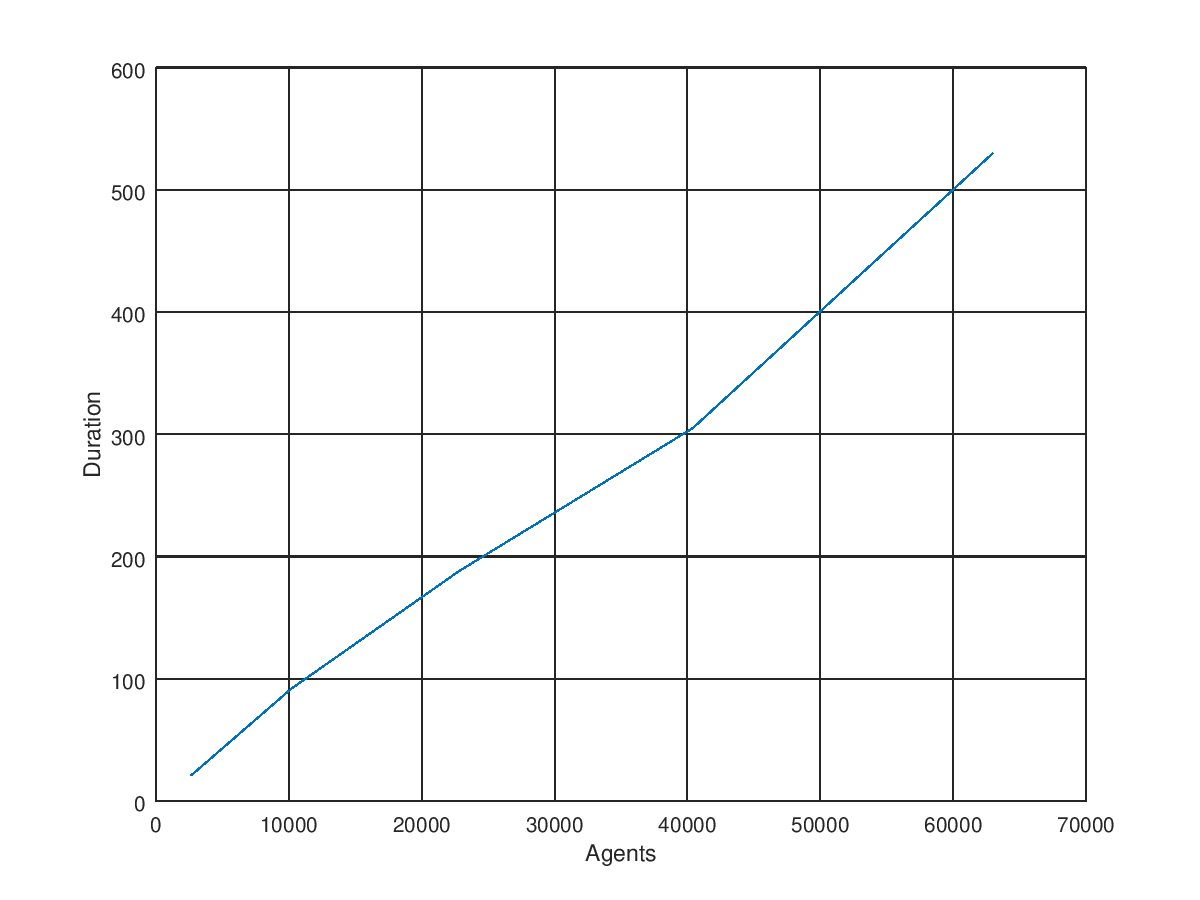
\includegraphics[width=0.6\textwidth, angle=0]{./fig/agents_duration_stm.png}
	\caption{Plot of Table \ref{tab:agent_by_duration}: agents by duration, exhibiting a clear linear trend in performance scaling.}
	\label{fig:agent_by_duration}
\end{figure}


Interpretation of the data leads to the following conclusions:
\begin{enumerate}
	%\item On a single core, no transaction retries should happen, the results support that assumption.
	\item Sharing state using an STM variable is much more time- and memory-efficient than using the State Monad.
	\item Running STM on multiple cores concurrently leads to a significant performance improvement.
	\item We get a linear performance scaling when using STM, which is remarkable because concurrent problems rarely scale linearly.
\end{enumerate}

\subsection{Comparison to Java RePast single core}
To have an idea where the functional implementation is performance-wise compared to the established object-oriented methods, we conducted a performance comparison with a Java implementation using RePast, running on a single-core. All parameters were the same and the simulation was run until virtual time t=100 was reached, on various grid-sizes. Due to the lack of proper timing facilities in RePast we measured the time by hand using a stopwatch. Although this is not very precise it gives a rough estimate and allows a very basic comparison, being precise enough if the difference is larger than 1 second. We measured the following:

\begin{center}
  \begin{tabular}{ l || c | r }
    Grid-Size & Java Repast & 4-Core Haskell \\ \hline \hline 
    51 x 51 & 10 sec & 20 sec \\ \hline
    101 x 101 & 110 sec & 103 sec \\ \hline
    201 x 201 & 1260 sec & 305 sec \\ \hline
  \end{tabular}
\end{center}

While on a 51x51 grid the single-core Java RePast version outperforms the 4-core Haskell STM version by about 200\%, the figure is inverted on a 201x201 grid where the 4-core Haskell STM version outperforms the single core Java Repast version by 400\%. We can conclude that the single-core Java RePast version clearly outperforms the Haskell STM 4-core version on small grid-sizes but that the Haskell STM version scales up with increasing grid-sizes and clearly outperforms the RePast version with increasing number of agents.

\section{Discussion}
\label{sect:stm_discussion}
Using STM for concurrent, large-scale ABS seems to be a very promising approach as our proof-of-concept has shown. The concurrency abstractions of STM are very powerful, yet simple enough to allow convenient implementation of concurrent agents without the nastiness of low level concurrent locks. Also we have shown by experiments, that we indeed get a very substantial speed-up and that we even got linear performance scaling for our model. 

Interestingly, STM primitives map nicely to ABS concepts: using a share environment through a \textit{TVar} is very easy, also we implemented in an additional proof-of-concept the use of \textit{TChan} which can be seen as persistent message boxes for agents, underlining the message-oriented approach found in many agent-based models. Also \textit{TChan} offers a broadcast transactional channel, which supports broadcasting to listeners which maps nicely to a pro-active environment or a central auctioneer upon which agents need to synchronize.

Running in STM instead of IO also makes the concurrent nature more explicit and at the same time restricts it to purely STM behaviour. So despite obviously losing the reproducibility property due to concurrency, we still can guarantee that the agents can't do arbitrary IO as they are restricted to STM operations only.

Depending on the nature of the transactions, retries could become a bottle neck. The central problem of STM is to keep the retries low, which is directly influenced by the read/writes on the STM primitives. By choosing more fine-grained / suitable data-structures e.g. using a TArray instead of an Array within a TVar, one can reduce retries significantly. We tracked the retries in our proof-of-concept using the stm-stats library and arrived at a ratio of 0.0\% retries - note that there were some retries but they were so low that they weren't significant.

\section{Further Research}
\label{sect:stm_further}
Our work on STM for ABS is only a proof-of-concept with promising results. Still there is more work needed:

\begin{itemize}
	\item So far we only looked at a time-driven model. It would be of fundamental interest whether we can somehow apply STM and concurrency to an event-driven approach as well. We hypothesise that it is not as striking and easy due to the fundamental sequential approach to even-processing. Generally one could run agents concurrently and undo actions when there are inconsistencies - something which STM supports out of the box.
	\item So far we only looked at asynchronous agent-interactions through TVar and TChan: agents modify the data or send a message but don't synchronise on a reply. Also a receiving agent doesn't do synchronised waiting for messages or data-changes. Still, in some models we need this synchronous way of agent-interactions where agents interact over multiple steps within the same global time-step. We yet have to come up with an easy-to-use solution for this problem using STM.
\end{itemize}